\documentclass{article}
\usepackage{amsmath}
\usepackage{amssymb}
\usepackage{graphicx}
\usepackage{hyperref}
\usepackage[version=4]{mhchem}


\begin{document}
\section*{Problem}
\(A B\) is the diameter of the semicircle as shown in the figure. \(C D\) \(\perp A B\), with the foot at \(D\). Two circles \(O_{1}\left(r_{1}=12\right)\) and \(O_{2}\left(r_{2}=8\right)\) inscribed in the semicircle and are tangent to \(C D\). The tangent points to \(A B\) are \(E_{1}\) and \(E_{2}\), respectively. Find the length of \(A B\).\\
\centering
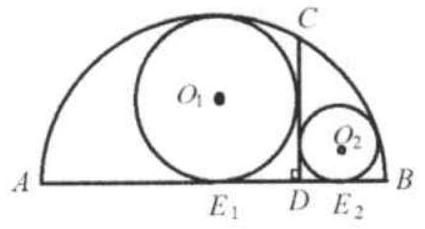
\includegraphics[width=\textwidth]{images/185(3).jpg}

\section*{Solution}
Connect \(O_{1} E_{1}\) and \(O_{2} E_{2}\).\\
\(E_{1} D=O_{1} E_{1}=12 . D E_{2}=O_{2} E_{2}=8\).\\
Let \(A D=x, D B=y\).\\
Then \(A E_{1}=x-12, E_{1} B=y+12, A E_{2}=x+8\), \(E_{2} B=y-8\).\\
\centering
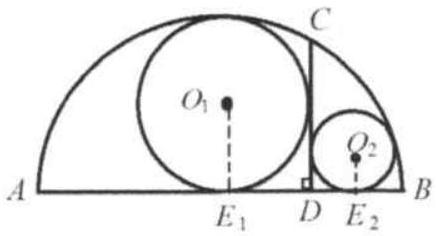
\includegraphics[width=\textwidth]{images/189(1).jpg}

Then we have \(\frac{1}{A E_{1}}+\frac{1}{E_{1} B}=\frac{1}{O_{1} E_{1}}\)

\[
\frac{1}{A E_{2}}+\frac{1}{E_{2} B}=\frac{1}{O_{2} E_{2}}
\]

Or \(\quad \frac{1}{x-12}+\frac{1}{y+12}=\frac{1}{12}\)

\[
\frac{1}{x+8}+\frac{1}{y-8}=\frac{1}{8}
\]

Solving we get \(x=32, y=18\).\\
\(A B=x+y=50\).

\end{document}
